\appendix
\chapter{Appendix}
\section{Implementation of the Framework} \label{implementation_framework}
%!+++++++++++++++++++++++++++++++++++++++++++++++++++++++++++++++++++++++++++++++++++++++++++++++++++++++++++++++++++++++
In this section, we will briefly discuss the working and functioning of each of the files present in the framework. Each of the files are crucial and responsible
for the proper functioning and execution of the framework. 

\subsection{Utility files}
During creation of a framework, it is common to repeat functionalities in different parts of the codebase. But, it is considered a bad practice in software development as 
it leads to code redundancy and makes the codebase difficult to maintain. Therefore, it is ideal to store the repeated functionalities in a separate file and
import them when required. A utility file refers to a Python source file  which contains utility functions or helper functions. These functions are built in a 
way that they can provide common functionalities or operate specific tasks which can be reused in different parts of the codebase. 
\begin{figure}[!ht] %! Image is not being displayed as expected. FIX IT!!!
  \centering
  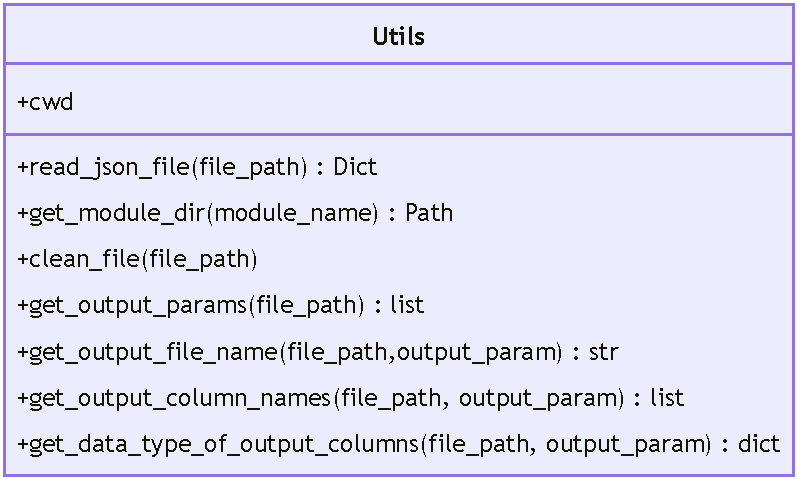
\includegraphics[width=0.6\textwidth]{Images/utils.pdf}
  \caption{Overview of functions in \texttt{utils.py}}

  \label{utils_overview}
\end{figure}

\textbf{\texttt{utils.py}} is a helper file which mainly consists of functions which are later used to build complex functions for the creation of the framework.
It consists of functions like \texttt{read\_json\_file} which reads a \acrshort{json} file and returns the data in the form of dictionary, get the path of a module,
get column names of a \texttt{csv} file, get data type of a column in a \texttt{csv} file and many more. Figure \ref{utils_overview} shows the functions present 
in the \texttt{utils.py} file.

\subsection{Creation and Execution of Parametric System}
Since the main objective of the framework is to automate the integration of modules when running parametric simulations, it is essential to create the parametric 
system automatically. The script \texttt{create\_parametric\_system.py} assists in creating the parametric system without the help of Optislang's GUI. The 
parametric system is created based on the information present in \texttt{module\_config.json}. The \acrshort{json} file consists of key-value pairs containing 
crucial information for creating the system, like name of the main script containing the algorithm, type of module to build, i.e, Python or MATLAB. 
%\begin{figure}[!ht]
%  \centering
%  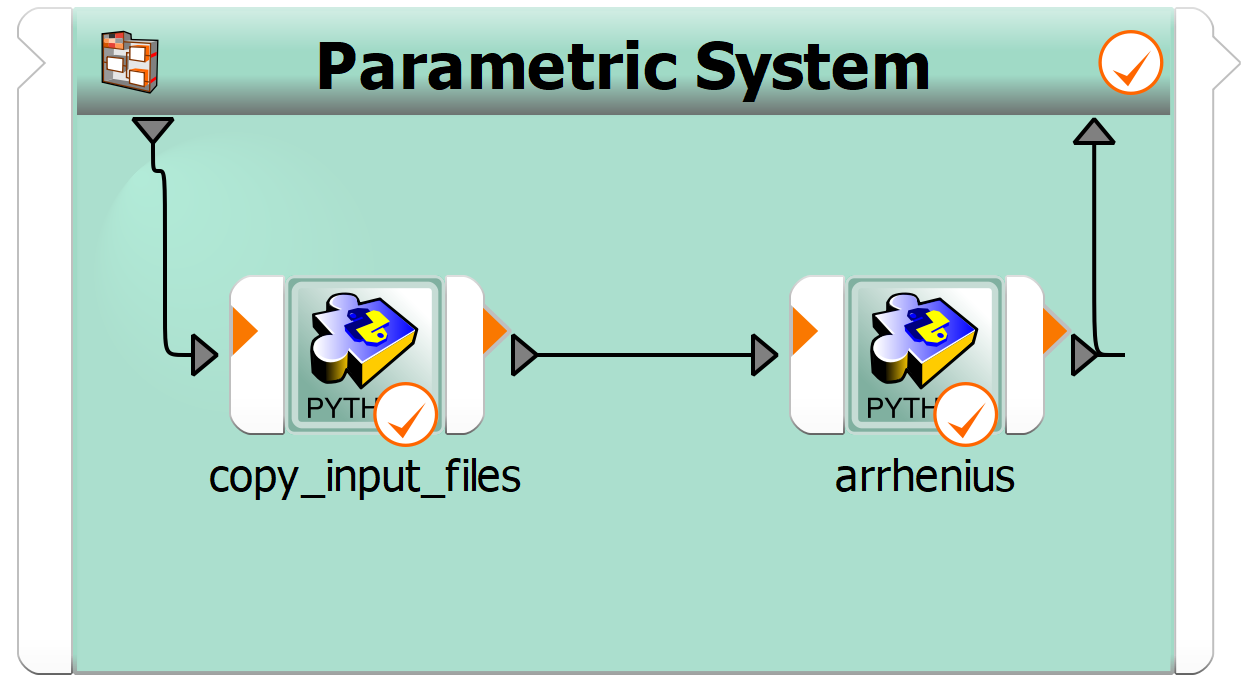
\includegraphics[width=0.5\textwidth]{Images/parametric_system_with_copy_actor.png}
%  \caption{Example of a parametric system with copy actor}
%  \label{parametric_system_with_copy_actor}
%\end{figure}

Optislang takes in different functions to create a system depending on the type of actor. Therefore, type of module is required. Since the framework is automated,
the process of inputting the requried files also needs to be automated. The script \texttt{input\_files.py} is responsible for retrieving the input files from 
OpenShift. 
After providing the input files, the parametric system is created. 

The next step is to run the created parametric system. \texttt{run\_parametric\_system.py} runs the newly created parametric system. This system is being run 
inside the Python interpreter provided by Optislang. These scripts are being called and ran in an orchestrated manner inside the class \texttt{ParametricSystem}.

\subsection{Framework Orchestration} \label{parametric_system_code}
For better code organization, reusability and encapsulation, the framework is built using classes. Classes are the pillar of object-oriented programming.
There are many advantages of using classes.
\begin{itemize}
  \item Code is maintained and organized in a better way.
  \item Data can be encapsulated and hidden from the user.
  \item Code can be reused and extended easily.
\end{itemize}
Creation of framework is possible by using the class \texttt{ParametricSystem}. Since the creation of framework is tedious and complex, we make use of 
\texttt{utils.py} which assists in building the class. Figure \ref{parametric_system_class} shows the functions present in the class \texttt{ParametricSystem}.
\begin{figure}[!ht]
  \centering
  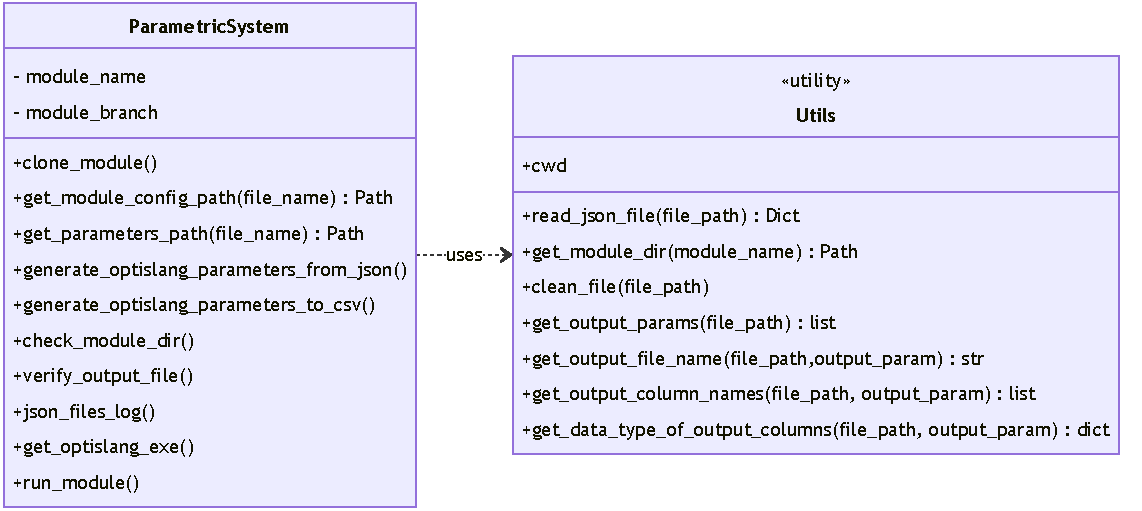
\includegraphics[width=0.9\textwidth]{Images/parametric_system_class.pdf}
  \caption{Overview of the class \texttt{ParametricSystem}}
  \label{parametric_system_class}
\end{figure}

The class takes in the arguments \texttt{module\_name} and \texttt{module\_branch} which are required to clone the module from GitHub. 
The following provides a high-level overview of the key functions used in the framework. These functions are essential for automating the process of testing 
standalone modules in Optislang.

\begin{itemize}
  \item \textbf{\texttt{clone\_module()}}:
  This function is responsible for cloning a module from a GitHub repository. It ensures that any existing module is deleted before cloning the new one, 
  thereby maintaining a clean working environment.

  \item \textbf{\texttt{get\_module\_config\_path()}}:
  This function retrieves the absolute path of the \texttt{module\_config.json} file. It takes the file name as an argument and returns its absolute path, 
  facilitating easy access to the configuration file.

  \item \textbf{\texttt{get\_parameters\_path()}}:
  Similar to \texttt{get\_module\_config\_path()}, this function returns the absolute path of the \texttt{parameters.json} file. It ensures that the framework 
  can locate and use the parameters file efficiently.

  \item \textbf{\texttt{generate\_optislang\_parameters\_to\_csv()}}:
  This function converts the parameters from the \texttt{parameters.json} file into a CSV format required by the parametric system. The resulting CSV file 
  is saved in the current working directory as \texttt{optislang\_actor\_parameters.csv}.

  \item \textbf{\texttt{generate\_optislang\_parameters\_from\_json()}}:
  This function generates the parameters needed for creating the parametric system from the \texttt{parameters.json} file. The parameters are saved in a Python 
  file, \texttt{optislang\_parameters.py}, which is later used in the system creation process.

  \item \textbf{\texttt{check\_module\_dir()}}:
  This function creates a mock directory structure to accommodate hardcoded paths within the modules. It ensures that the necessary directories and files are 
  in place, allowing the modules to function correctly.

  \item \textbf{\texttt{verify\_output\_files()}}:
  This function verifies the existence and correctness of the output files generated by the parametric system. It is used after the system is created to ensure 
  that the output meets the expected criteria.
  \begin{figure}[!ht]
    \centering
    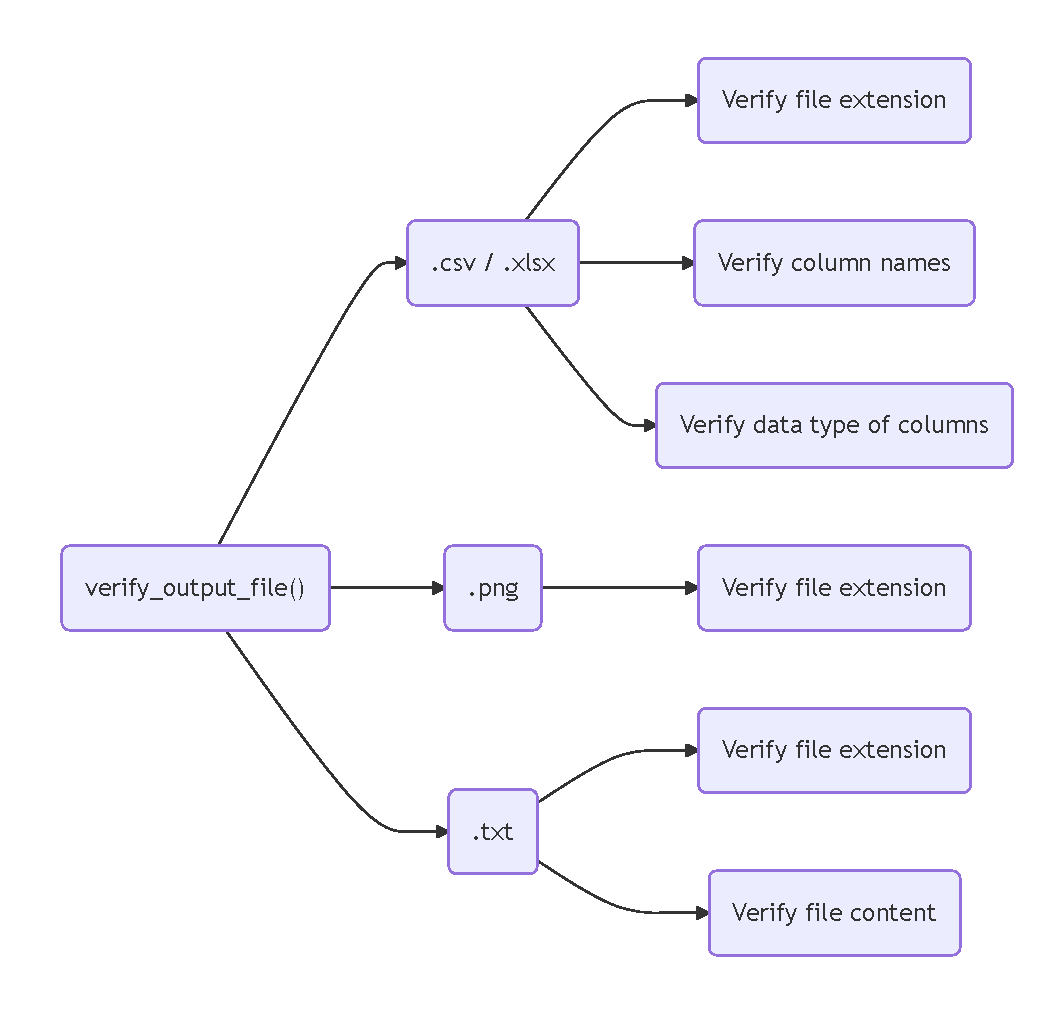
\includegraphics[width=0.7\textwidth]{Images/verify_output_file.pdf}
    \caption{Working of \texttt{verify\_output\_files()} function}
    \label{verify_output_files}
  \end{figure}
  
  To verify the output, we first retrieve the verification data from \texttt{module\_config.json}, which includes properties like column names, file names, 
  formats, and data types. The function iterates through the output folder to check the presence of all output files. Using the Pandas library, it reads 
  \texttt{csv} files to verify column names and data types. If all checks pass, a success message is displayed; otherwise, an error message specifies the issue.

  For non-\texttt{csv} files, the function also verifies the presence and correctness of \texttt{.txt} and \texttt{.png} files. For \texttt{.txt} files, it 
  additionally checks if the file is not empty. Figure \ref{verify_output_files} shows the working of \texttt{verify\_output\_files()} function.
\end{itemize}

%! Is a section of implementation of FastAPI required?